\chapter{Fundamentação teórica}
\label{Fundamentação teórica}

Esse capitulo oferece uma visão abrangente e detalhada de temas cruciais em cardiologia e tecnologia, começando com uma explanação aprofundada sobre a Anatomia e Fisiologia do Coração na Seção \ref{sec:Anatomia e fisiologia da coração}. Esta Seção descreve minuciosamente a estrutura do coração, enfatizando qsuas câmaras e funções no sistema cardiovascular, além de discutir condições patológicas como a insuficiência cardíaca.  Em seguida, o Capítulo se aprofunda no uso da Ultrassonografia e o Ecocardiograma na medicina na Seção \ref{sec:A ultra sonografia e o ecocardiograma}. Esta parte do texto cobre os princípios físicos da ultrassonografia, detalhando o papel dos diferentes tipos de transdutores e a relevância da técnica na obtenção de imagens cardíacas detalhadas. A Seção \ref{sec:Ecocardiograma} dedicada especificamente ao Ecocardiograma expandindo o tema, explorando sua aplicação na avaliação detalhada da função e estrutura cardíacas, incluindo métodos de medição e análise ecocardiográfica. A última Seção do Capítulo faz a transição para um campo distinto, introduzindo o conceito de Redes Neurais artificiais. Aqui, o foco é estabelecer uma base sólida sobre o que são as Redes Neurais Artificiais (RNAs), explorando suas semelhanças com o funcionamento cerebral humano e sua capacidade de aprendizado e processamento de informações. Esta introdução às redes neurais estabelece a base para discussões mais avançadas sobre suas arquiteturas e aplicações específicas, sem adentrar em detalhes sobre modelos específicos como as redes Transformer e convolucionais será discutido detalhadamente no capitulo \ref{Revisão bibliográfica}. A abordagem é  estruturada para oferecer um entendimento claro e conciso sobre a relevância e o funcionamento das RNAs, preparando o terreno para discussões mais profundas em Capítulos subsequentes.

\section{Anatomia e fisiologia do coração}
\label{sec:Anatomia e fisiologia da coração}

O coração desempenha um importante papel no transporte sanguíneo pelo sistema cardiovascular. É um órgão aproximadamente do tamanho de um punho, situado ligeiramente à esquerda do esterno, composto por quatro câmaras interligadas. Entre elas, o átrio direito recebe o sangue das veias e o encaminha para o ventrículo direito. O ventrículo direito, por sua vez, envia o sangue para os pulmões, onde é enriquecido com oxigênio. O átrio esquerdo recebe o sangue oxigenado dos pulmões e o direciona para o ventrículo esquerdo. Este último, o ventrículo esquerdo, é a câmara mais robusta, sendo responsável por bombear o sangue rico em oxigênio para todo o corpo. Essas contrações vigorosas do ventrículo esquerdo desempenham um papel fundamental na manutenção da pressão sanguínea \cite{Tortora2023-wk}.

Todavia, quando o funcionamento do coração é comprometido, surge uma síndrome clínica conhecida como insuficiência cardíaca. Essa condição pode ser originada por diversos fatores, afetando estruturas como o pericárdio, o miocárdio, o endocárdio, as válvulas cardíacas, os grandes vasos ou, até mesmo, apresentar origem em anormalidades metabólicas \cite{YANCY2013e147}. Os principais sintomas associados à insuficiência cardíaca incluem dispneia, fadiga e retenção de líquidos, podendo resultar em congestão em órgãos como os pulmões e o sistema esplâncnico, bem como causar edema periférico. A insuficiência cardíaca é geralmente diagnosticada com base na história clínica do paciente e no exame físico, sendo notável a sua predominância na afetação da função do ventrículo esquerdo \cite{YANCY2013e147}.

\textcite{FOLSE1962} demonstraram que a relação entre o volume sistólico (VS) e o volume diastólico final (VDF) poderia fornecer informações significativas para uma análise hemodinâmica da função ventricular esquerda. No contexto da insuficiência cardíaca, um parâmetro crítico é a fração de ejeção (FEVE), que quantifica a porcentagem de sangue expulsa do ventrículo esquerdo a cada batimento cardíaco. 

De acordo com \textcite{Zipes2006-ke} a fração de ejeção do ventrículo esquerdo (FEVE) é essencial para a avaliação da função ventricular, sendo crucial para diferenciar a Insuficiência Cardíaca com Fração de Ejeção Preservada (ICFEP) da Insuficiência Cardíaca com Fração de Ejeção Reduzida (ICFER). A ICFEP ocorre quando o ventrículo esquerdo mantém uma fração de ejeção normal, mas apresenta dificuldades no relaxamento e enchimento durante a diástole, levando a sintomas de insuficiência cardíaca apesar de uma FEVE aparentemente normal. Por outro lado, a ICFER é caracterizada por uma fração de ejeção reduzida, indicando que o ventrículo esquerdo não está bombeando sangue de forma eficiente, resultando em um menor volume de sangue sendo ejetado a cada batimento cardíaco. A FEVE é calculada pela razão entre a diferença do volume diastólico final (VDF) e o volume sistólico final (VSF) pelo VDF, conforme ilustrado na equação \ref{eq:feve}

\begin{equation}
\label{eq:feve}
FEVE = \frac{EDV - ESV}{EDV}.
\end{equation}

A Figura \ref{fig:card} ilustra vários frames do ciclo cardíaco capturados por imagens de ecocardiograma. Estas imagens são utilizadas para estimar o EDV e o ESV. O frame diastólico mostra o ventrículo esquerdo totalmente cheio de sangue (EDV), enquanto o frame sistólico mostra o ventrículo após a contração (ESV). A análise desses frames permite calcular a FEVE, oferecendo uma visão detalhada da dinâmica cardíaca em pacientes com insuficiência cardíaca.


\begin{figure}[H]
\centering
 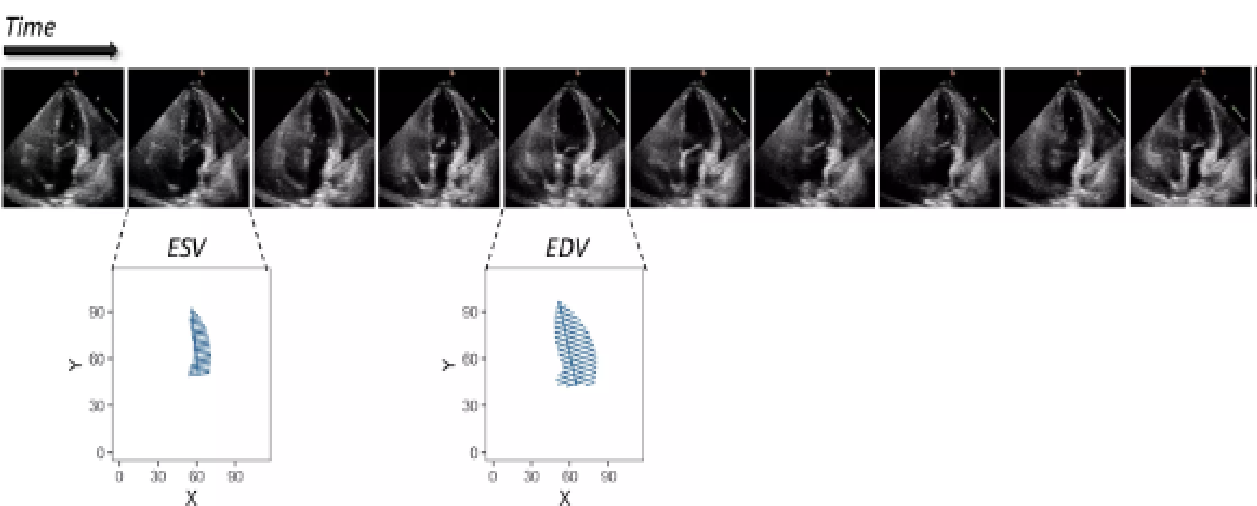
\includegraphics[width=1\linewidth]{capitulos//figuras/saidadoeco.png}
\caption{Frames representativos do ciclo cardíaco demonstrando o volume diastólico final e o volume sistólico final, usados para o cálculo da fração de ejeção de \textcite{Ouyang2020}.}
\label{fig:card}
\end{figure}


\section{A ultrasonografia e o ecocardiograma}
\label{sec:A ultra sonografia e o ecocardiograma}

A ecografia utiliza ondas sonoras do tipo ultrassônicas para criar imagens de estruturas internas do corpo humano \cite{9781496321282}. Na física, o termo "ultra-som" se aplica a toda energia acústica com frequência acima da audição humana (20.000 hertz ou 20 kilohertz) \cite{Carovac2011}. No diagnóstico médico, o ultrassom é usado como pulsos com frequência entre 3 e 10 MHz \cite{velavan}.

Essas ondas sonoras, quando utilizadas em ecografia, são caracterizadas por parâmetros essenciais que descrevem sua natureza. Estes incluem o comprimento de onda ($\Lambda$), que representa o comprimento da onda em metros, a frequência (\textit{f}), medida em Hertz, e a velocidade do ultrassom, que é aproximadamente 1540 m/s nos tecidos moles (v) \cite{Carovac2011}. O relacionamento entre a frequência (f), a velocidade e o comprimento de onda ($\lambda$) pode ser descrito pela Equação \eqref{eq:relacao}.

\begin{equation}
v = f \lambda
\label{eq:relacao}
\end{equation}


No contexto da ecografia, é importante ressaltar que as ondas de ultrassom são ondas mecânicas que requerem um meio físico para sua propagação \cite{Humphrey2007}. A complexa estrutura dos tecidos humanos torna-os heterogêneos, permitindo a observação de fenômenos como reflexão, refração e espalhamento das ondas sonoras\cite{velavan}.

 A formação de imagens por ultrassom é um processo  que se baseia na habilidade de mapear o nível de som retroespalhado em tons de cinza \cite{49500}. Para compreender a física por trás das imagens de ultrassom, é essencial examinar o comportamento do feixe sonoro ao interagir com o meio \cite{Papalo2019}.

Em suma, a capacidade do ultrassom em gerar imagens está diretamente ligada à reflexão e ao espalhamento das ondas sonoras nos contornos dos órgãos e em tecidos heterogêneos, causado pelas diferenças na impedância acústica \cite{Papalo2019}. Esse fenômeno permite a visualização de estruturas subcutâneas no corpo, incluindo tendões, músculos, articulações, vasos sanguíneos e órgãos internos, tornando possível a detecção de patologias ou lesões \cite{Papalo2019}.

 O ultrassom utilizado na área médica é gerado em materiais cristalinos especiais que, quando eletricamente excitados, têm a capacidade de vibrar em frequências extremamente altas, da ordem de milhões de vibrações por segundo. Os dispositivos que produzem e detectam o ultrassom são denominados transdutores \cite{ISBN9241592990}.

Os transdutores utilizados na ultrassonografia são fabricados a partir de materiais piezoelétricos. Esses materiais reagem à aplicação de uma diferença de potencial nos eletrodos de sua superfície, gerando uma deformação mecânica direcionada. Curiosamente, esse fenômeno pode ser observado de maneira inversa, onde a aplicação de uma força mecânica na superfície do material resulta na geração de uma voltagem nos eletrodos \cite{biscegli_2003}.


Na área médica, o transdutor de ultrassom, também conhecido como sonda ecoscópica, é um dispositivo inserido no corpo do paciente que contém um ou mais transdutores de ultrassom, conforme explicado por \textcite{Carovac2011}. A aplicação do ultrassom envolve uma variedade de tipos de transdutores, e a escolha do transdutor a ser utilizado depende do órgão ou tecido específico que será examinado, como destacado por \textcite{ufersa}. Os principais tipos de transdutores incluem o transdutor curvo ou convexo, que é usado em exames de órgãos internos como fígado, vesícula biliar, rins, feto, útero, ovários e coração; o transdutor linear, destinado a exames de órgãos externos e superficiais, incluindo tireoide, mamas, testículos, músculos, tendões e pele; o transdutor endocavitário, adequado para exames de órgãos internos através das vias naturais do corpo (esôfago, vagina, reto) ou durante cirurgias abertas ou fechadas; o transdutor setorial, usado principalmente para facilitar o exame de órgãos internos, como o coração e o cérebro; e transdutores especiais que utilizam tecnologias adicionais, como volumétrica e matricial, para obter imagens especiais, como 3D/4D e biplanares.


Os sinais elétricos produzidos pelos cristais piezoelétricos do transdutor são enviados a um amplificador e demonstrados no monitor com intensidades proporcionais à sua energia, permitindo que sejam decodificados por diferentes modos como o modo-A, modo-B e modo-M . O modo A do ultrassom consiste em uma imagem unidimensional exibida como uma série de picos verticais, que correspondem à profundidade das estruturas encontradas nos diferentes tecidos. A distância entre os picos ecoados pode ser calculada dividindo-se a velocidade do ultrassom no tecido (1540 m/s) pela metade do tempo decorrido, embora forneça poucas informações sobre a relação espacial das estruturas fotografadas. O modo B, amplamente utilizado na medicina, opera com vários cristais no transdutor que são acionados em sequência, realizando uma varredura de feixes de ultrassom que formam uma imagem bidimensional. Já o modo M é produzido por um único feixe em uma varredura de ultrassom para produzir uma imagem que exibe sinais de movimento, onde o movimento de uma estrutura, como uma válvula cardíaca, pode ser representado de maneira ondulatória \cite{ufersa}.

\section{Ecocardiograma}
\label{sec:Ecocardiograma}

A ultrassonografia cardíaca, também conhecida como ecocardiograma, é um dos exames mais empregados no diagnóstico de doenças cardíacas devido à sua natureza não invasiva, custo acessível e ampla disponibilidade. Na prática clínica, a ecocardiografia desempenha um papel fundamental na avaliação de cardiopatias, determinação do tamanho das câmaras cardíacas, avaliação de massas ventriculares, diagnóstico de valvopatias e análise da hemodinâmica do coração \cite{8520425232}.

\textcite{Mitchell2019-br} explica que para a aquisição de imagens bidimensionais do coração transtorácico, são definidas nomenclaturas que define planos, visões e manobras de varredura para a obtenção de imagens ecocardiográficas conforme Figura \ref{fig:planos}. Os movimentos do transdutor são descritos em relação aos eixos anterior, posterior, superior, inferior, lateral e medial. Todos os transdutores possuem uma marcação que determina a orientação. As janelas de varredura consideradas incluem paraesternal (localização do transdutor próximo ao esterno no peito), apical (localização do transdutor abaixo da mama esquerda, perto do ápice do coração), subcostal (posicionamento do transdutor abaixo do esterno, melhor obtido com o paciente deitado de costas) e supraesternal (posicionamento do transdutor acima do esterno, mostrando o arco aórtico) como descrito na Figura \ref{fig:planos2} . 

Para a aquisição das janelas paraesternal e apical, o paciente é posicionado em decúbito lateral esquerdo. Na projeção paraesternal em eixo longo (PLAX), a marcação do índice de localização aponta para o ombro direito do paciente. Já na visão paraesternal em eixo curto (PSAX), a marcação aponta para o ombro esquerdo, proporcionando imagens em plano axial. A janela apical é localizada abaixo da mama esquerda, permitindo a visualização do ápice cardíaco\cite{Mitchell2019-br} .

 
 \begin{figure}[H]
   \centering
   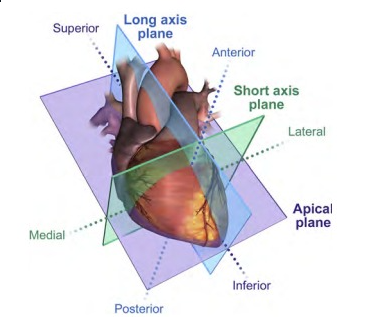
\includegraphics[width=0.6\linewidth]{capitulos/figuras/planos.png}
   \caption{Nomenclaturas que define planos, visões e manobras de varredura para a obtenção de imagens ecocardiográficas. Retirado de \textcite{Mitchell2019-br}}
   \label{fig:planos}
\end{figure}

 \begin{figure}[H]
   \centering
   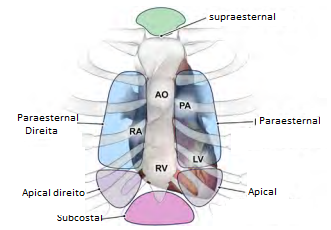
\includegraphics[width=0.6\linewidth]{capitulos/figuras/planos2.png}
   \caption{Nomenclaturas que define janelas ecocardiográficas. Imagens de \textcite{Mitchell2019-br}.}
   \label{fig:planos2}
\end{figure}

No contexto desta dissertação, a avaliação do tamanho do ventrículo esquerdo (VE) desempenha um papel crucial na análise da função cardíaca usando ecocardiograma. Essa avaliação envolve a utilização de parâmetros que incluem dimensões lineares internas e volumes do VE, obtidos tipicamente no final da diástole e da sístole. 
Esses parâmetros são essenciais para determinar a fração de ejeção cardíaca, um indicador crítico da função cardíaca. As medidas lineares, preferencialmente obtidas no corte paraesternal de eixo longo representados na Figura \ref{fig:parasternal}, requerem cuidadosa colocação do cursor eletrônico para evitar secções oblíquas do ventrículo, enquanto as medidas volumétricas, baseadas em traçados das interfaces entre o miocárdio e a cavidade, são mais precisas do que os cálculos lineares que assumem uma forma geométrica fixa do VE \cite{Lang2015}. 

\begin{figure}[H]
\centering
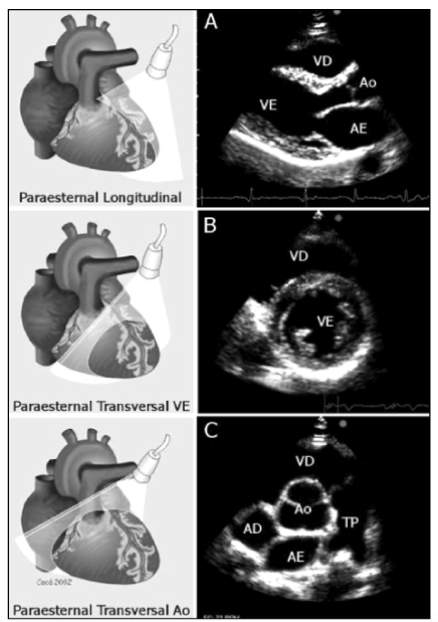
\includegraphics[width=0.6\linewidth]{capitulos/figuras/paraesternalC.png}
\caption{Corte Paraesternal de Eixo Longo do Ventrículo Esquerdo, imagem de \textcite{Silva2004}.}
\label{fig:parasternal}
\end{figure}

\textcite{Lang2015} indica que para medições volumétricas precisas, é aconselhável obter volumes a partir dos cortes apicais quatro e duas câmaras, maximizando as áreas do VE e evitando o encurtamento do ventrículo esquerdo, o que poderia resultar em uma subestimação do volume.

\begin{figure}[H]
\centering
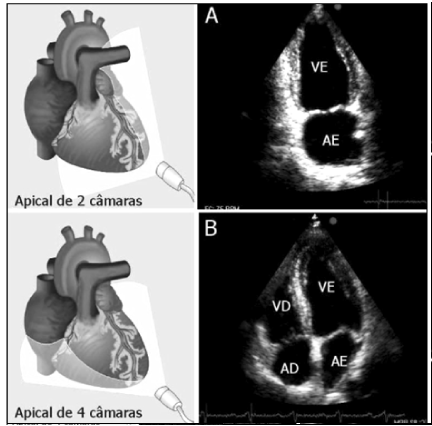
\includegraphics[width=0.6\linewidth]{capitulos/figuras/Apical.png}
\caption{Representação da técnica de Simpson para ecocardiograma apical de 4 câmaras e de 2 câmaras \textcite{Lang2015} }
\label{fig:apical}
\end{figure}

A estimativa do volume do ventrículo esquerdo (VE) pode ser adquirida tanto por meio da ecocardiografia bidimensional (E2D) quanto da ecocardiografia tridimensional (E3D). No contexto da E2D, o método predominante para calcular o volume do VE é o conhecido método biplanar da soma de discos conforme Figura \ref{fig:figsimpsom}.

\begin{figure}[H]
\centering
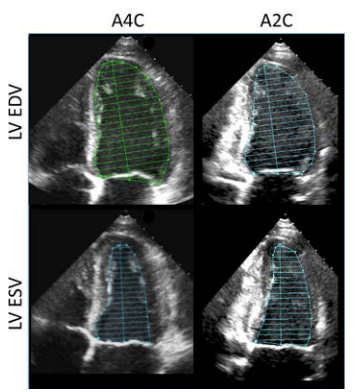
\includegraphics[width=0.3\linewidth]{capitulos/figuras/simpsons.png}
\caption{Representação da técnica de Simpson para ecocardiograma apical de 4 câmaras e de 2 câmaras, \textcite{Lang2015})}
\label{fig:figsimpsom}
\end{figure}


Como alternativa viável  o método área-comprimento na Figura \ref{fig:figcomprimento}, o qual presume que o VE possui uma forma semelhante à de um projétil. Nesse método, a área da seção transversal do VE no terço médio do corte paraesternal de eixo-curto é calculada, e o comprimento do ventrículo é estimado a partir do ponto médio do plano anular no corte apical de quatro câmaras, ressaltando que a suposição da forma de projétil nem sempre é precisa, esse método é mostrado na Figura\ref{fig:3d}.


\begin{figure}[H]
\centering
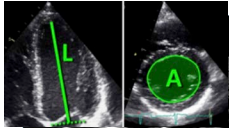
\includegraphics[width=0.3\linewidth]{capitulos/figuras/comprimento.png}
\caption{Representação da técnica do método área-comprimento, retirado de \textcite{Lang2015}.}
\label{fig:figcomprimento}
\end{figure}

\begin{figure}[H]
\centering
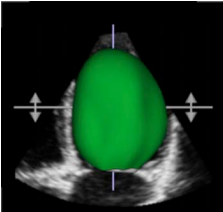
\includegraphics[width=0.3\linewidth]{capitulos/figuras/3d.png}
\caption{Representação da técnica por medição do volume por meio da ecocardiografia tridimensional (E3D) por \textcite{Lang2015}}
\label{fig:3d}
\end{figure}


 Os valores normais para parâmetros ecocardiográficos 2D relacionados ao tamanho do ventrículo esquerdo e sua função, segmentados de acordo com o sexo dos pacientes. Esses valores, detalhados na Tabela \ref{tab:echoparams}, incluem médias e variações de dois desvios padrão (2SD) para cada parâmetro, tanto para homens quanto para mulheres. As variações de 2SD fornecem um intervalo importante, indicando onde se espera encontrar aproximadamente 95\% das medições para uma distribuição normal dos dados.

\begin{table}[htbp]
\centering
\small % Diminui a fonte da tabela
\caption{Parâmetros Ecocardiográficos}
\label{tab:echoparams}
\begin{tabular}{lcccc}
\toprule
Parâmetro & \multicolumn{2}{c}{Homens} & \multicolumn{2}{c}{Mulheres} \\
\cmidrule(lr){2-3} \cmidrule(lr){4-5}
& Média ± DP & Variação 2DP & Média ± DP & Variação 2DP \\
\midrule
Dimensão Diastólica Interna (mm) & 50.2 ± 4.1 & 42.0-58.4 & 45.0 ± 3.6 & 37.8-52.2 \\
Dimensão Sistólica Interna (mm) & 32.4 ± 3.7 & 25.0-39.8 & 28.2 ± 3.3 & 21.6-34.8 \\
Volume Diastólico Final (mL) & 106 ± 22 & 62-150 & 76 ± 15 & 46-106 \\
Volume Sistólico Final (mL) & 41 ± 10 & 21-61 & 28 ± 7 & 14-42 \\
Volume Diastólico Final (mL/m²) & 54 ± 10 & 34-74 & 45 ± 8 & 29-61 \\
Volume Sistólico Final (mL/m²) & 21 ± 5 & 11-31 & 16 ± 4 & 8-24 \\
Fração de Ejeção (\%) & 62 ± 5 & 52-72 & 64 ± 5 & 54-74 \\
\bottomrule
\end{tabular}
\end{table}



A Tabela \ref{tab:severidade_ve} mostra as faixas de valores normais e pontos de corte de graus de severidade para a fração de ejeção do ventrículo esquerdo, derivados do ecocardiograma 2DE, segmentados por sexo. Essas faixas são úteis na avaliação da função cardíaca e na identificação de anomalias, permitindo que profissionais de saúde e pesquisadores determinem o grau de severidade de possíveis problemas cardíacos em pacientes do sexo masculino e feminino \cite{Lang2015}.

\begin{table}[htbp]
\centering
\caption{Faixa de Valores Normais e Pontos de Corte de Graus de Severidade para a Fração de Ejeção do Ventrículo Esquerdo Derivados do 2DE.}
\label{tab:severidade_ve}
\begin{tabular}{lcc}
\toprule
\textbf{Parâmetros} & \textbf{Homem} & \textbf{Mulher} \\
\midrule
Faixa Levemente normal & 52 - 72 & 54 - 74 \\
Anormal & 41 - 51 & 41 - 53 \\
Moderadamente anormal & 30 - 40 & 30 - 40 \\
Gravemente anormal & <30 & <30 \\
\bottomrule
\end{tabular}
\end{table}

\section{Redes neurais artificiais}
\label{sec:Redes neurais}

Segundo \textcite{haykin2001redes}, as Redes Neurais Artificiais (RNAs) são sistemas de processamento paralelos compostos por unidades simples, capazes de armazenar conhecimento e utilizá-lo no futuro. Embora haja ainda muito a ser compreendido sobre o funcionamento neurofisiológico dos neurônios e suas conexões, as RNAs compartilham características fundamentais com o cérebro. Elas extraem conhecimento do ambiente por meio de um processo de aprendizagem ou treinamento, e os pesos sinápticos, que representam as conexões entre os neurônios, são utilizados para armazenar o conhecimento adquirido.

Essas semelhanças entre as RNAs e o cérebro destacam-se em sua capacidade de adquirir conhecimento do ambiente através de aprendizagem e treinamento, além do armazenamento desse conhecimento nos pesos sinápticos. No entanto, é importante reconhecer que a fidelidade desses modelos em relação à fisiologia real ainda é limitada devido à complexidade do funcionamento neurofisiológico. A pesquisa em RNAs envolve diversas disciplinas, como neurofisiologia, psicologia, física, computação, engenharia e estatística, permitindo uma abordagem multidisciplinar para explorar todo o potencial dessas redes neurais artificiais \cite{haykin2001redes}.


\textcite{haykin2001redes} descreve que as redes neurais artificiais são construídas com base em modelos matemáticos inspirados pela cognição humana e pela neurobiologia, contendo vários pressupostos essenciais. Primeiramente, assumimos que o processamento da informação ocorre por meio de elementos chamados neurônios. Cada neurônio recebe sinais de entrada, realiza cálculos internos e gera um sinal de saída, sendo estes neurônios artificiais análogos aos neurônios biológicos encontrados no cérebro humano. Além disso, os neurônios nas redes neurais artificiais são interconectados por meio de conexões que permitem a transmissão dos sinais de um neurônio para outro, com cada conexão possuindo um peso associado que representa a importância relativa dessa conexão na transmissão do sinal. Os pesos sinápticos são ajustados durante o processo de aprendizado para otimizar o desempenho da rede. No que se refere à transmissão do sinal, em uma rede neural típica, a transmissão de sinal de um neurônio para o próximo é ponderada pelo peso sináptico associado à conexão entre eles, determinando a contribuição relativa desse sinal na ativação do neurônio de destino. Ou seja, alguns sinais podem ter mais influência do que outros com base nos pesos sinápticos correspondentes. Cada neurônio, ou unidade, em uma rede neural artificial possui também uma função de ativação, que recebe a soma ponderada dos sinais de entrada e produz a saída do neurônio. Geralmente, as funções de ativação são não-lineares, permitindo que a rede modele relações complexas entre os dados.

Incorporando todos os elementos mencionados por \textcite{CHAI2021100134}, as redes neurais artificiais demonstram uma  habilidade para aprender e discernir padrões  a partir dos dados de entrada. Esta capacidade de processar informações multifacetadas e adaptar-se de forma autônoma as torna extremamente valiosas em diversas aplicações, incluindo classificação, previsão e reconhecimento de padrões. Devido a essa versatilidade, elas são essenciais em campos variados, como visão computacional, processamento de linguagem natural (NLP), reconhecimento de voz e de vídeo, além de serem amplamente utilizadas no setor financeiro e bancário.

No centro dessa revolução tecnológica, destacam-se várias arquiteturas de rede neural, cada uma com características e aplicações específicas na visão computacional. Entre as mais proeminentes estão as Redes Neurais Convolucionais (CNNs), Redes Neurais Recorrentes (RNNs), Redes Adversárias Gerativas (GANs), Redes de Função de Base Radial (RBFNs), Perceptrons Multicamadas (MLPs), Mapas Auto-Organizáveis (SOMs), Redes de Crenças Profundas (DBNs), Máquinas Boltzmann Restritas (RBMs) e Autoencoders. Cada uma dessas arquiteturas oferece abordagens únicas e especializadas, contribuindo significativamente para os avanços e desafios da visão computacional \cite{CHAI2021100134}.

Neste contexto, o próximo Capítulo, \ref{Revisão bibliográfica}, explorará a aplicação de redes neurais profundas na avaliação da função cardíaca utilizando vídeos de ecocardiograma, analisando e discutindo trabalhos relevantes nesse campo. 
